\documentclass{mimosis}

\usepackage{metalogo}

%%%%%%%%%%%%%%%%%%%%%%%%%%%%%%%%%%%%%%%%%%%%%%%%%%%%%%%%%%%%%%%%%%%%%%%%
% Some of my favourite personal adjustments
%%%%%%%%%%%%%%%%%%%%%%%%%%%%%%%%%%%%%%%%%%%%%%%%%%%%%%%%%%%%%%%%%%%%%%%%
%
% These are the adjustments that I consider necessary for typesetting
% a nice thesis. However, they are *not* included in the template, as
% I do not want to force you to use them.

% This ensures that I am able to typeset bold font in table while still aligning the numbers
% correctly.
\usepackage{etoolbox}
\usepackage{lipsum}

\usepackage{color}
\definecolor{myred}{rgb}{0.8588,0.2667,0.2157}
\newcommand{\TODO}[1]{\color{myred} \textbf{#1} \color{black}}

\usepackage[binary-units=true]{siunitx}
\DeclareSIUnit\px{px}

\sisetup{%
  detect-all           = true,
  detect-family        = true,
  detect-mode          = true,
  detect-shape         = true,
  detect-weight        = true,
  detect-inline-weight = math,
}

%%%%%%%%%%%%%%%%%%%%%%%%%%%%%%%%%%%%%%%%%%%%%%%%%%%%%%%%%%%%%%%%%%%%%%%%
% Hyperlinks & bookmarks
%%%%%%%%%%%%%%%%%%%%%%%%%%%%%%%%%%%%%%%%%%%%%%%%%%%%%%%%%%%%%%%%%%%%%%%%

\usepackage[%
  colorlinks = true,
  citecolor  = RoyalBlue,
  linkcolor  = RoyalBlue,
  urlcolor   = RoyalBlue,
  ]{hyperref}

\usepackage{bookmark}

%%%%%%%%%%%%%%%%%%%%%%%%%%%%%%%%%%%%%%%%%%%%%%%%%%%%%%%%%%%%%%%%%%%%%%%%
% Bibliography
%%%%%%%%%%%%%%%%%%%%%%%%%%%%%%%%%%%%%%%%%%%%%%%%%%%%%%%%%%%%%%%%%%%%%%%%
%
% I like the bibliography to be extremely plain, showing only a numeric
% identifier and citing everything in simple brackets. The first names,
% if present, will be initialized. DOIs and URLs will be preserved.

\usepackage[%
  autocite     = plain,
  backend      = bibtex,
  doi          = true,
  url          = true,
  giveninits   = true,
  hyperref     = true,
  maxbibnames  = 99,
  maxcitenames = 99,
  sortcites    = true,
  style        = numeric,
  ]{biblatex}

%%%%%%%%%%%%%%%%%%%%%%%%%%%%%%%%%%%%%%%%%%%%%%%%%%%%%%%%%%%%%%%%%%%%%%%%
% Some adjustments to make the bibliography more clean
%%%%%%%%%%%%%%%%%%%%%%%%%%%%%%%%%%%%%%%%%%%%%%%%%%%%%%%%%%%%%%%%%%%%%%%%
%
% The subsequent commands do the following:
%  - Removing the month field from the bibliography
%  - Fixing the Oxford commma
%  - Suppress the "in" for journal articles
%  - Remove the parentheses of the year in an article
%  - Delimit volume and issue of an article by a colon ":" instead of
%    a dot ""
%  - Use commas to separate the location of publishers from their name
%  - Remove the abbreviation for technical reports
%  - Display the label of bibliographic entries without brackets in the
%    bibliography
%  - Ensure that DOIs are followed by a non-breakable space
%  - Use hair spaces between initials of authors
%  - Make the font size of citations smaller
%  - Fixing ordinal numbers (1st, 2nd, 3rd, and so) on by using
%    superscripts

% Remove the month field from the bibliography. It does not serve a good
% purpose, I guess. And often, it cannot be used because the journals
% have some crazy issue policies.
\AtEveryBibitem{\clearfield{month}}
\AtEveryCitekey{\clearfield{month}}

% Fixing the Oxford comma. Not sure whether this is the proper solution.
% More information is available under [1] and [2].
%
% [1] http://tex.stackexchange.com/questions/97712/biblatex-apa-style-is-missing-a-comma-in-the-references-why
% [2] http://tex.stackexchange.com/questions/44048/use-et-al-in-biblatex-custom-style
%
\AtBeginBibliography{%
  \renewcommand*{\finalnamedelim}{%
    \ifthenelse{\value{listcount} > 2}{%
      \addcomma
      \addspace
      \bibstring{and}%
    }{%
      \addspace
      \bibstring{and}%
    }
  }
}

% Suppress "in" for journal articles. This is unnecessary in my opinion
% because the journal title is typeset in italics anyway.
\renewbibmacro{in:}{%
  \ifentrytype{article}
  {%
  }%
  % else
  {%
    \printtext{\bibstring{in}\intitlepunct}%
  }%
}

% Remove the parentheses for the year in an article. This removes a lot
% of undesired parentheses in the bibliography, thereby improving the
% readability. Moreover, it makes the look of the bibliography more
% consistent.
\renewbibmacro*{issue+date}{%
  \setunit{\addcomma\space}
    \iffieldundef{issue}
      {\usebibmacro{date}}
      {\printfield{issue}%
       \setunit*{\addspace}%
       \usebibmacro{date}}%
  \newunit}

% Delimit the volume and the number of an article by a colon instead of
% by a dot, which I consider to be more readable.
\renewbibmacro*{volume+number+eid}{%
  \printfield{volume}%
  \setunit*{\addcolon}%
  \printfield{number}%
  \setunit{\addcomma\space}%
  \printfield{eid}%
}

% Do not use a colon for the publisher location. Instead, connect
% publisher, location, and date via commas.
\renewbibmacro*{publisher+location+date}{%
  \printlist{publisher}%
  \setunit*{\addcomma\space}%
  \printlist{location}%
  \setunit*{\addcomma\space}%
  \usebibmacro{date}%
  \newunit%
}

% Ditto for other entry types.
\renewbibmacro*{organization+location+date}{%
  \printlist{location}%
  \setunit*{\addcomma\space}%
  \printlist{organization}%
  \setunit*{\addcomma\space}%
  \usebibmacro{date}%
  \newunit%
}

% Display the label of a bibliographic entry in bare style, without any
% brackets. I like this more than the default.
%
% Note that this is *really* the proper and official way of doing this.
\DeclareFieldFormat{labelnumberwidth}{#1\adddot}

% Ensure that DOIs are followed by a non-breakable space.
\DeclareFieldFormat{doi}{%
  \mkbibacro{DOI}\addcolon\addnbspace
    \ifhyperref
      {\href{http://dx.doi.org/#1}{\nolinkurl{#1}}}
      %
      {\nolinkurl{#1}}
}

% Use proper hair spaces between initials as suggested by Bringhurst and
% others.
\renewcommand*\bibinitdelim {\addnbthinspace}
\renewcommand*\bibnamedelima{\addnbthinspace}
\renewcommand*\bibnamedelimb{\addnbthinspace}
\renewcommand*\bibnamedelimi{\addnbthinspace}

% Make the font size of citations smaller. Depending on your selected
% font, you might not need this.
\renewcommand*{\citesetup}{%
  \biburlsetup
  \small
}

\DeclareLanguageMapping{english}{english-mimosis}

\addbibresource{report.bib}

%%%%%%%%%%%%%%%%%%%%%%%%%%%%%%%%%%%%%%%%%%%%%%%%%%%%%%%%%%%%%%%%%%%%%%%%
% Fonts
%%%%%%%%%%%%%%%%%%%%%%%%%%%%%%%%%%%%%%%%%%%%%%%%%%%%%%%%%%%%%%%%%%%%%%%%

\ifxetexorluatex
  \setmainfont{Minion Pro}
\else
  \usepackage[lf]{ebgaramond}
  \usepackage[oldstyle,scale=0.7]{sourcecodepro}
  \singlespacing
\fi

\renewcommand{\th}{\textsuperscript{\textup{th}}\xspace}

\makeindex
\makeglossaries

%%%%%%%%%%%%%%%%%%%%%%%%%%%%%%%%%%%%%%%%%%%%%%%%%%%%%%%%%%%%%%%%%%%%%%%%
% Incipit
%%%%%%%%%%%%%%%%%%%%%%%%%%%%%%%%%%%%%%%%%%%%%%%%%%%%%%%%%%%%%%%%%%%%%%%%

\title{\texttt{Visualizing Music with Generative Adverserial Networks}}
\subtitle{Project report for the summer course of Deep Vision 2019}
\author{Peter Hügel and Florian Fallenbüchel}

\begin{document}
  \frontmatter

  \sloppy
  \begin{titlepage}
  \vspace*{5cm}
  \makeatletter
  \begin{center}
    \begin{Huge}
      \@title
    \end{Huge}\\[0.1cm]
    %
    \begin{Large}
      \@subtitle
    \end{Large}\\
    %
    \emph{by}\\
    \@author
  \end{center}
  \makeatother
\end{titlepage}


  \chapter{Abstract}
    \TODO{\lipsum[1]}

  \tableofcontents

  \mainmatter
  \sloppy

  \chapter{Introduction}
  In this project we wanted to generate visualizations of music tracks with the help of generative adverserial networks (GAN). 
  Our goal was for the visualizations to visibly correlate to the music when played alongside.
  For this we extract different sets of features from the music and use these features as seeds for the generators of our GANs, which we train on sets of real world images, flowers for the most part.\\
  For the feature extraction, we mainly tried out three different approaches. First, we generated mel spectrograms from the music and used these directly as input. 
  As our second approach, we reduced the size of the mel spectrograms with an autoencoder to then use the encoded vectors as input, and the last approach was to use the featuremap of an intermediate layer of a convolutional recurrent neural network (CRNN), trained to classify the genre of a given song from its corresponding mel spectrogram.\\
  For our GANs, we had two main architectures which we tried out during the project: deep convolutional generative adverserial networks (DCGAN), which enable us to train the generator in an unsupervised manner, and InfoGANs, which are an extension of DCGANs with the addition of maximizing
  the mutual information between a subset of the latent input vector and the observation.\\
  In the following sections we will explain our different approaches in detail and discuss their varying performance. We will start with the feature extraction, before we go into detail about our GANs until we finally talk about the results.

  \TODO{introduce the datasets}

  \chapter{Related Work}
    \lipsum

  \chapter{Feature Extraction}


  \chapter{Image Generation with GANs}
    In this chapter we elaborate on the different methods we employed to produce images from the extracted features. An arbitrary dataset of images can be used here, we went with \citetitle{102flower}~\cite{102flower}, a dataset of 102 different types of flowers containing slightly over 8000 images with a resolution of at least 500x500.
    
    \section{DCGAN}

    \section{InfoGAN}

  \chapter{Video Generation}\label{ch:results}

    In this chapter we combine the methods from the previous chapters. We also elaborate on some further preprocessing during the generation of videos. Finally we do our best to provide some results on paper.

    \section{Generating videos}
        
        Theoretically we can generate videos with each possible combination of extracted features and trained generators. The process is quite simple, the input song(s) are processed and melspectrograms are created. Depending on the chosen combination the melspectrograms are then used raw, encoded with the autoencoder, or processed through the CRNN. We then end up with 60 latent vectors per second of video, this information is used to create an image for each of those samples. From there we simply call ffmpeg to combine the images into a video, which is then combined with the input song.

    \section{Ensuring smooth transitions}
        
        Depending on the input song the resulting videos flickered and had very rapid and dramatic changes of images. As two very close latent vectors will produce a very similar image, the idea is to slow down our movement in the latent space. We realized this by implementing a gaussian smoothing with variable size. So depending on the song we can apply more or less smoothing.
        
        One might assume that the beginnning of change in an image should correlate with the beginning of change in sound. With this assumption we want to avoid smoothening future latent vectors into an image. Therefore we implemented a kernel that falls off very quickly in the direction of positive time, this results in a more smooth and slower movement through the latent space. For spikes in the song that only last a few frames, this smoothening will cause us to never reach the corresponding point within the latent space. Instead we move in the direction of that point but turn around / away before reaching it. More complex methods could be applied to shape our path through the latent space. For example, our path could be described using Bézier curve.

    \section{Results}

        Figure~\ref{fig:dcgan_samples} displays a collection of images that were generated with a DCGAN. We can observe that this particular model, which was using the raw melspectrograms as latent vector, manages to generate a wide variety of different flowers.

        \begin{figure}[ht]
            \centering
            \includegraphics[width=.94\textwidth]{images/fake_samples_not_cherry_picked}
            \caption[not used]
            {
                \textbf{A collection of images that were generated with a DCGAN. The latent vectors used to produce these images were randomly sampled from the music dataset.}
            }
            \label{fig:dcgan_samples}
        \end{figure}
        
        \newpage
        In figure~\ref{fig:video} we show a section of a melspectrogram and the images generated from that section. The images displayed here were produced without any smoothening techniques. Some images that showed little to no change have been omitted. A selection of example videos can be found here~\cite{examples}.

        \begin{figure}[ht!]
            \centering
            \fbox{
                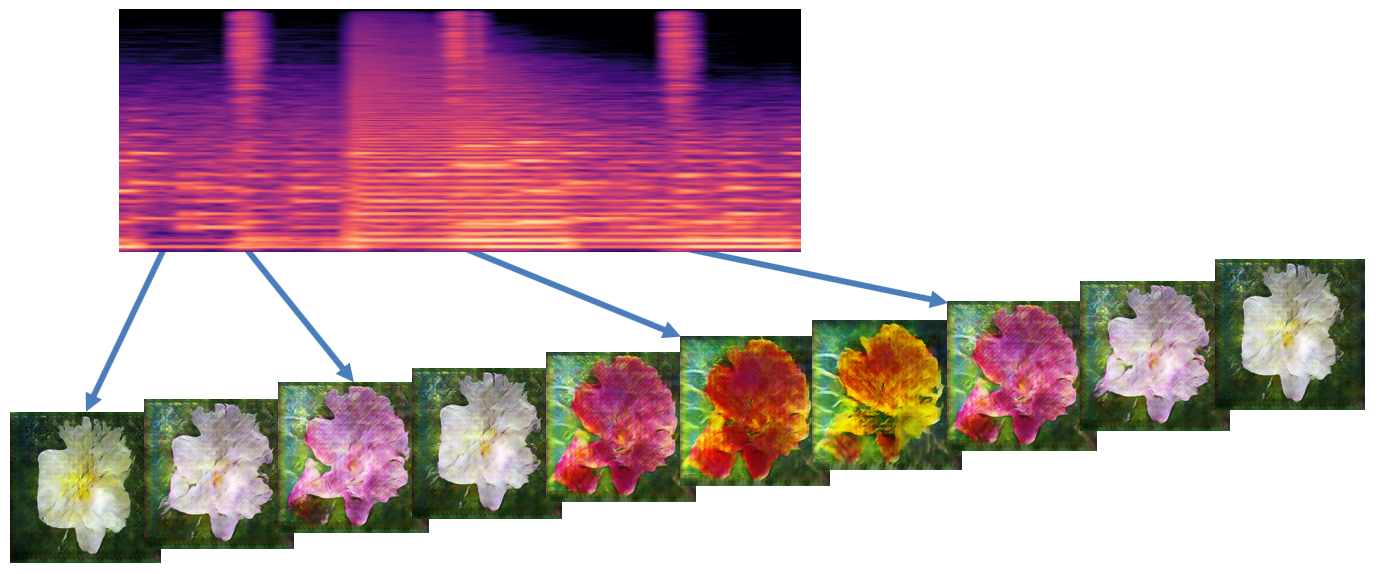
\includegraphics[width=.94\textwidth]{images/video_on_paper}
            }
            \caption[not used]
            {
                \textbf{An attempt at visualizing a resulting video on paper. We have connected the individual frames in the video with the underlying spectrogram. We can observe that similar sections in the melspectrogram produce very similar flower images.}
            }
            \label{fig:video}
        \end{figure}

        \section{Visualizing your own music}
            If the reader of this report would like to generate a visualization of a music track of his likings, he can download a compact version of a pretrained generator from our Google Drive~\cite{visualizer}. After extracting the zip file, one can place their desired mp3 file in the $song\_in$ folder and execute either \textit{start\_cuda.sh} or \textit{start\_cpu.sh}, if your device does not support cuda (warning, this can take very long). We currently only support the video generation directly from the mel spectrograms due to the mixed results of the other approaches. The script will then automatically calculate the mel spectrogram of the given song, apply a Gaussian smoothing over the time steps, feed the vectors to the pretrained generator and afterwords compile the images to a single video with the song added as the audio track. The resulting video will appear in the $song\_out$ folder adjacent to the $song\_in$ folder after everything is completed. If you would like to experiment with the smoothing, you can either change the kernel size with the \textit{smooth\_count} parameter, or disable smoothing entirely by removing the \textit{smooth} parameter from the respective bash scripts. The whole procedure requires a variety of python packages, as well as ffmpeg installed on the system. We cannot guarantee that every genre will deliver satisfying results, an average metal song seemed to throw off the results quite a bit, but maybe you have some fun with the generators.

  \chapter{Conclusion}

    We reached our base goal of generating visualizations that visibly correlate to the music when played alongside each other. We achieved our best results with the generator that was trained with the raw mel spectrogram as latent vectors. When applying our smoothing techniques during the video generation we have also achieved our secondary goal of having smooth transitions. Depending on the song those techniques do not necessarily have to be applied for a smooth result.

    There are many things we still want to try or investigate. We want to try different combinations of complexities regarding the generator and discriminator. Instead of randomly taking one sample from each song per epoch during training of the GANs it should at least be modified to randomly select one sample from all songs in each step. Another option would be to construct a distribution of the samples from which we can then generate samples as needed.
    
    While the individual images of the combination of encoded features and InfoGAN look promising, the problem of images being very similar is still unsolved. Because the training takes multiple days before a judgement can be made it is very tedious and time-consuming. To prevent this issue in the future we would take a look at ProGANs where the output resolution is slowly increased during training. This significantly speeds up the training at the beginning and one is no longer required to decide on the final resolution from the start.

    Further, we would like to test around more with the features from the CRNN, as they seemed promising at first, already involving some smoothing of the features through the convolutions. A model with a much more consistent performance would be the first step to counter the varying results, as well as calculating a distribution from the different feature maps for training, to have a smooth feature space for the generators. At last, there are still a variety of image datasets on which we want to train our generators, eventually producing more diverse visualizations.

% This ensures that the subsequent sections are being included as root
% items in the bookmark structure of your PDF reader.
\bookmarksetup{startatroot}
\backmatter

	\begingroup
		\let\clearpage\relax
		\glsaddall
		% \printglossary[type=\acronymtype]
		% \newpage
		\printglossary
		\newpage
		\listoffigures
	\endgroup

	\printindex
	\printbibliography

\end{document}
